\documentclass[xcolor=pdftex,romanian,colorlinks]{beamer}

\usepackage[export]{adjustbox}
\usepackage{../tslides}
\usepackage[all]{xy}
\usepackage{pgfplots}
\usepackage{flowchart}
\usetikzlibrary{arrows,positioning,calc}
\lstset{language=Haskell}
\lstset{escapeinside={(*@}{@*)}}

\AtBeginSection[]{
  \begin{frame}
  \vfill
  \centering
  \begin{beamercolorbox}[sep=8pt,center,shadow=true,rounded=true]{title}
    \usebeamerfont{title}\insertsectionhead\par%
  \end{beamercolorbox}
  \vfill
  \end{frame}
}


\title[PD---Meta-Programare]{Programare declarativă}

\subtitle{Functori, functori aplicativi, monoizi\thanks{bazat pe \emph{\href{http://learnyouahaskell.com/functors-applicative-functors-and-monoids}{Learn You a Haskell for Great Good}}}}

\begin{document}
\begin{frame}
  \titlepage
\end{frame}

\section{Cutii și computații}

\begin{frame}[fragile]{Tipuri parametrizate --- „cutii”}
\begin{block}{Idee}
O clasă largă de tipuri parametrizate pot fi gândite ca „cutii”, recipiente care pot conține elemente de tipul dat ca argument.
\end{block}
\vfill
\begin{block}{Exemple}
\begin{itemize}
\item Clasa de tipuri opțiune asociază unui tip \lstinline$a$, tipul \lstinline$Maybe a$
\begin{itemize}
\item cutii goale: \lstinline$Nothing$
\item cutii care țin un element \lstinline$x$ de tip \lstinline$a$: \lstinline$Just x$
\end{itemize}
\item Clasa de tipuri listă asociază unui tip \lstinline$a$, tipul \lstinline$[a]$
\begin{itemize}
\item cutii care țin 0, 1, sau mai multe elemente de tip \lstinline$a$: \lstinline$[1, 2, 3]$, \lstinline$[]$, \lstinline$[5]$
\end{itemize}
\end{itemize}
\end{block}
\end{frame}


\begin{frame}[fragile]{Tipuri parametrizate --- „cutii”}
\begin{block}{Idee}
O clasă largă de tipuri parametrizate pot fi gândite ca „cutii”, recipiente care pot conține elemente de tipul dat ca argument.
\end{block}
\vfill
\begin{block}{Exemplu: tip de date pentru arbori binari}
\begin{asciihs}
data Arbore a = Nil
              | Nod a Arbore Arbore
\end{asciihs}
\begin{itemize}
\item Un arbore este o „cutie” care poate ține 0, 1, sau mai multe elemente de tip \lstinline$a$:

\lstinline$Nod 3 Nil (Nod 4 (Nod 2 Nil Nil) Nil)$, \lstinline$Nil$, \lstinline$Nod 3 Nil Nil$
\end{itemize}
\end{block}
\end{frame}

\begin{frame}[fragile]{Generalizare: Tipuri parametrizate --- „computații”}
\begin{block}{Idee}
O clasă largă de tipuri parametrizate pot fi gândite ca „contexte computaționale”: computații care, atunci când se execută, pot produce rezultate de tipul dat ca argument.
\end{block}
\vfill
\begin{block}{Exemple}
\begin{itemize}
\item \lstinline$Maybe a$ descrie rezultate de computații deterministe care pot eșua
\begin{itemize}
\item computații care eșuează: \lstinline$Nothing$
\item computații care produc un element de tipul dat: \lstinline$Just 4$
\end{itemize}
\item \lstinline$[Int]$ descrie liste de rezultate posibile ale unor computații nedeterministe 
\begin{itemize}
\item care pot produce oricare dintre rezultatele date: \lstinline$[1, 2, 3]$, \lstinline$[]$, \lstinline$[5]$
\end{itemize}
\end{itemize}
\end{block}
\end{frame}

\begin{frame}[fragile]{Tipuri parametrizate --- „computații”}
\begin{block}{Idee}
O clasă largă de tipuri parametrizate pot fi gândite ca „contexte computaționale”: computații care, atunci când se execută, pot produce rezultate de tipul dat ca argument.
\end{block}
\vfill
\begin{block}{Exemple}
\begin{itemize}
\item \lstinline$IO a$ descrie computații care atunci când se execută produc rezultate de tip \lstinline$a$
\begin{itemize}
\item \lstinline$getLine :: IO String$, \lstinline$getChar :: IO Char$
\end{itemize}
\item \lstinline$Either e a$ descrie rezultate de tip a ale unor computații deterministe care pot eșua cu o eroare de tip $e$
\begin{itemize}
\item \lstinline$Right 5 :: Either e Int$ reprezintă rezultatul unei computații reușite
\item \lstinline$Left "OOM" :: Either String a$ reprezintă o excepție de tip \lstinline$String$
\end{itemize}
\end{itemize}
\end{block}
\end{frame}


\begin{frame}[fragile]{Tipuri parametrizate --- „computații”}
\begin{block}{Idee}
O clasă largă de tipuri parametrizate pot fi gândite ca „contexte computaționale”: computații care, atunci când se execută, pot produce rezultate de tipul dat ca argument.
\end{block}
\begin{block}{Exemplu: tipul funcțiilor de sursă dată}
\begin{itemize}
\item \lstinline$t -> a$ descrie computații care atunci când primesc o intrare de tip \lstinline$t$ produc un rezultat de tip \lstinline$a$
\begin{itemize}
\item \lstinline$(++ "!") :: String -> String$ este o computație care dat fiind un șir, îi adaugă un semn de exclamare
\item \lstinline$length :: String -> Int$ este o computație care dat fiind un șir, îi prduce lungimea acestuia
\item \lstinline$id :: String -> String$ este o computație care produce șirul dat ca argument
\end{itemize}
\end{itemize}
\end{block}
\end{frame}

\begin{frame}[fragile]{Clase de tipuri pentru cutii și computații?}
\begin{block}{Întrebare}
Care sunt trăsăturile comune ale acestor tipuri parametrizate care pot fi gândite intuitiv ca cutii care conțin elemente / computații care produc rezultate?
\end{block}
\vfill
\begin{block}{Problemă}
Putem proiecta clase de tipuri care descriu funcționalități comune tuturor acestor tipuri?
\end{block}
\end{frame}

\section{Functori}

\begin{frame}[fragile]{Problemă}
\begin{block}{Formulare cu cutii}
Dată fiind o funcție \lstinline$f :: a -> b$ și o cutie \lstinline$ca$ care conține elemente de tip \lstinline$a$, vreau să să obțin o cutie \lstinline$cb$ care conține elemente de tip \lstinline$b$ obținute prin transformarea elementele din cutia \lstinline$ca$ folosind funcția \lstinline$f$ (și doar atât!)
\end{block}

\begin{block}{Formulare cu computații}
Dată fiind o funcție \lstinline$f :: a -> b$ și o computație \lstinline$ca$ care produce rezultate de tip \lstinline$a$, vreau să să obțin o computație \lstinline$cb$ care produce rezultate de tip \lstinline$b$ obținute prin transformarea rezultatelor produse de computația \lstinline$ca$ folosind funcția \lstinline$f$ (și doar atât!)
\end{block}

\begin{block}{Exemplu --- liste}
Dată fiind o funcție \lstinline$f :: a -> b$ și o listă $la$ de elemente de tip \lstinline$a$, vreau să să obțin o lista  de elemente de tip \lstinline$b$ transformând fiecare element din $la$ folosind funcția \lstinline$f$ (și doar atât!)
\end{block}

\end{frame}

\begin{frame}[fragile]{Clasa de tipuri Functor}
\begin{block}{Definiție}
\begin{asciihs}
class Functor f where
  fmap :: (a -> b) -> f a -> f b
\end{asciihs}

Dată fiind o funcție \lstinline$f :: a -> b$ și \lstinline$ca :: f a$, \lstinline$fmap$ produce \lstinline$cb :: f b$ \color{gray}{obținută prin transformarea rezultatelor produse de computația \lstinline$ca$ folosind funcția \lstinline$f$ (și doar atât!)}

\end{block}
\vfill
\begin{block}{Instanță pentru liste}
\begin{asciihs}
instance Functor [] where
  fmap = map
\end{asciihs}
\end{block}
\end{frame}

\begin{frame}[fragile]{Clasa de tipuri Functor}{Instanțe}
\begin{asciihs}
class Functor f where
  fmap :: (a -> b) -> f a -> f b
\end{asciihs}
\vfill
\begin{block}{Instanță pentru tipul optiune \lstinline$fmap :: (a -> b) -> Maybe a -> Maybe b$}
\onslide<2>
\begin{asciihs}
instance Functor Maybe where
  fmap f Nothing = Nothing
  fmap f (Just x) = Just (f x)
\end{asciihs}
\end{block}
\vfill
\onslide<1->
\begin{block}{Instanță pentru tipul arbore \lstinline$fmap :: (a -> b) -> Arbore a -> Arbore b$}
\onslide<2>
\begin{asciihs}
instance Functor Arbore where
  fmap f Nil = Nil
  fmap f (Nod x l r) = Nod (f x) (fmap f l) (fmap f r)
\end{asciihs}
\end{block}
\end{frame}

\begin{frame}[fragile]{Clasa de tipuri Functor}{Instanțe}
\begin{asciihs}
class Functor f where
  fmap :: (a -> b) -> f a -> f b
\end{asciihs}
\vfill
\begin{block}{Instanță pentru tipul eroare \lstinline$fmap :: (a -> b) -> Either e a -> Either e b$}
\onslide<2>
\begin{asciihs}
instance Functor (Either e) where
    fmap _ (Left x) = Left x
    fmap f (Right y) = Right (f y)
\end{asciihs}
\end{block}
\vfill
\onslide<1->
\begin{block}{Instanță pentru tipul funcție \lstinline$fmap :: (a -> b) -> (t -> a) -> (t -> b)$}
\onslide<2>
\begin{asciihs}
instance Functor (->) a where
  fmap f g = f . g  -- sau, mai simplu, fmap = (.)
\end{asciihs}
\end{block}
\end{frame}


\begin{frame}[fragile]{Clasa de tipuri Functor}{Instanțe}
\begin{asciihs}
class Functor f where
  fmap :: (a -> b) -> f a -> f b
\end{asciihs}
\vfill
\begin{block}{Instanță pentru tipul I/O \lstinline$fmap :: (a -> b) -> IO a -> IO b$}
\begin{itemize}
\item Folosind notația \lstinline$do$
\onslide<2>
\begin{asciihs}
instance Functor IO where
  fmap f ioa = do
     x <- ioa
     return (f x)
\end{asciihs}

\onslide<1->
\item Folosind operatorul de legare
\onslide<2>
\begin{asciihs}
  fmap f ioa = ioa >>= (\ x -> return (f x))
\end{asciihs}
\item Sau, mai scurt,
\begin{asciihs}
  fmap f ioa = ioa >>= (return . f)
\end{asciihs}
\end{itemize}
\end{block}
\end{frame}

\begin{frame}[fragile]{Exemple}
\begin{asciihs}
Main> fmap (*2) [1..3]

Main> fmap (*2) (Just 200) 

Main> fmap (*2) Nothing  

Main> fmap (*2) (+100) 4

Main> fmap (*2) (Right 6)

Main> fmap (*2) (Left 1)

Main> fmap (show . (*2) . read) getLine  >>=  putStrLn
\end{asciihs}
\end{frame}

\begin{frame}[fragile]{Exemple}
\begin{asciihs}
Main> fmap (*2) [1..3]
[2,4,6]
Main> fmap (*2) (Just 200) 
Just 400
Main> fmap (*2) Nothing  
Nothing
Main> fmap (*2) (+100) 4
208
Main> fmap (*2) (Right 6)
Right 12
Main> fmap (*2) (Left 135)
Left 135
Main> fmap (show . (*2) . read) getLine  >>=  putStrLn
123
246
\end{asciihs}
\end{frame}


\begin{frame}{Proprietăți ale functorilor}
\begin{itemize}
\item Argumentul \lstinline$f$ al lui \lstinline$Functor f$ definește o transformare de tipuri 
\begin{itemize}
\item \lstinline$f a$ este tipul \lstinline$a$ transformat prin functorul \lstinline$f$
\end{itemize}
\item \lstinline$fmap$ definește transformarea corespunzătoare a funcțiilor
\begin{itemize}
\item \lstinline$fmap :: (a -> b) -> $\alert{\lstinline$($}\lstinline$f a -> f b$\alert{\lstinline$)$}
\end{itemize}
\end{itemize}
\begin{block}{Contractul lui \lstinline$fmap$}
\begin{itemize}
\item \structure{\lstinline$fmap f ca$} e obținută prin transformarea rezultatelor produse de computația \lstinline$ca$ folosind funcția \lstinline$f$ (și doar atât!)
\item Abstractizat prin două legi:
\begin{description}
\item[identitate] \lstinline$fmap id == id$
\item[compunere] \lstinline$fmap (f . g) == fmap f . fmap g$
\end{description}
\end{itemize}
\end{block}

\end{frame}

\section{Categorii și Functori}

\begin{frame}[fragile]{Categorii}
O categorie $\mathbb{C}$ este dată de:
\begin{itemize}
\item O clasă $|\mathbb{C}|$ a \structure{obiectelor} 
\item Pentru oricare două obiecte $A, B \in |\mathbb{C}|$, 

o mulțime $\mathbb{C}(A,B)$ a \structure{săgeților} „de la $A$ la $B$”

$f\in \mathbb{C}(A,B)$ poate fi scris ca $f : A \rightarrow B$ 
\item Pentru orice obiect $A$ o săgeată $\mathit{id}_A : A \rightarrow A$ numită \structure{identitatea} lui $A$
\item Pentru orice obiecte $A$, $B$, $C$, o operație de compunere a săgeților
$\circ : \mathbb{C}(B,C) \times \mathbb{C}(A,B) \rightarrow \mathbb{C}(A,C)$
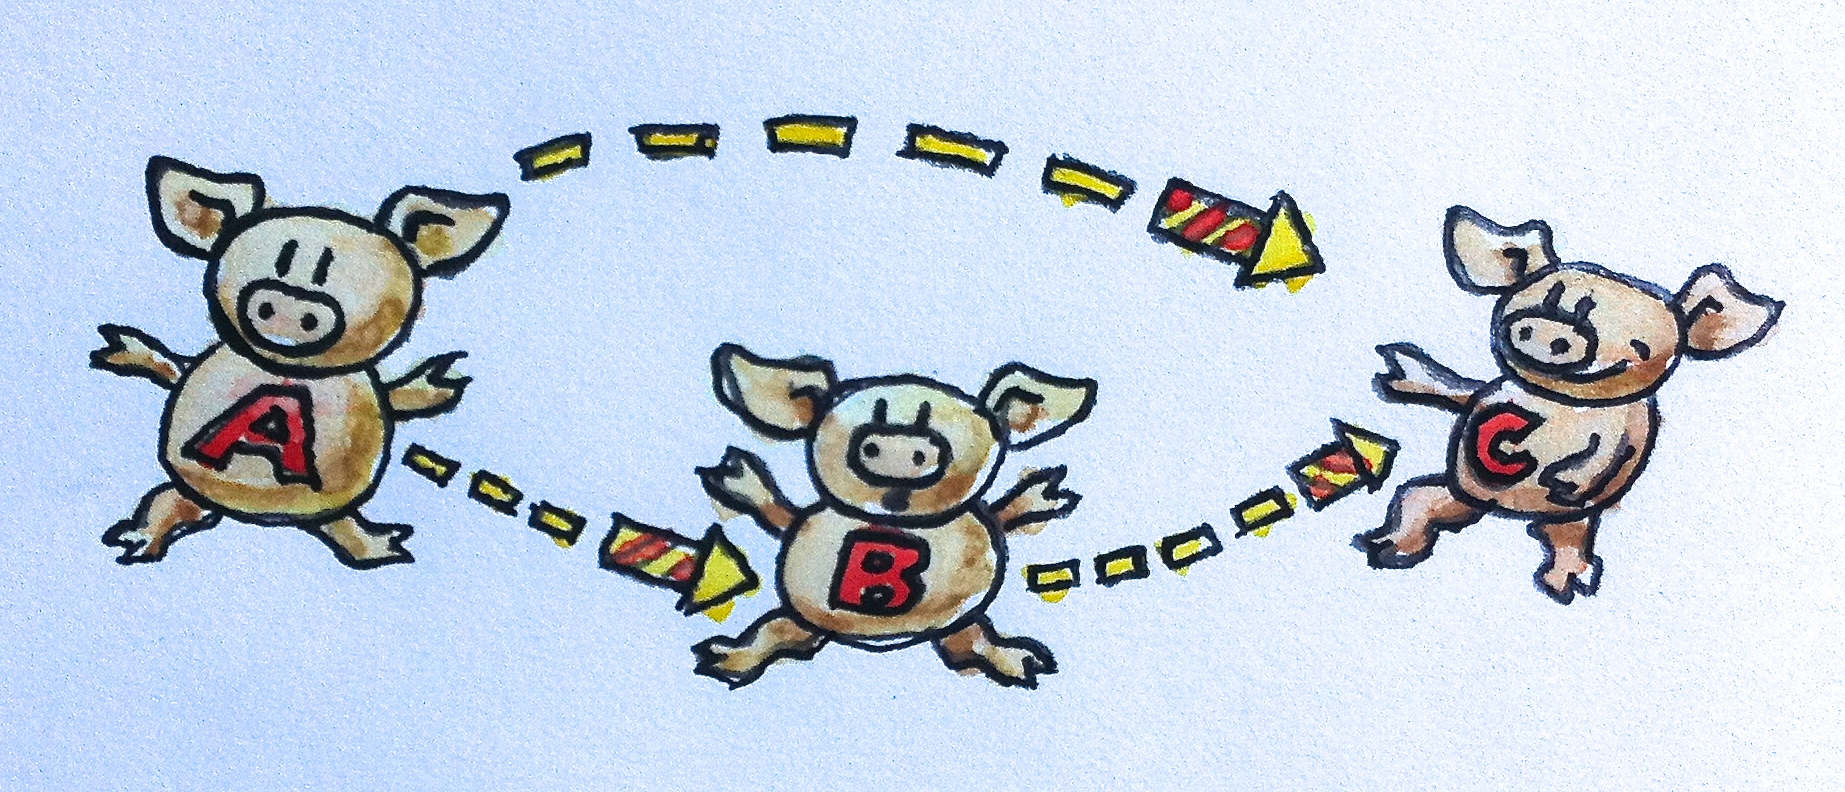
\includegraphics[scale=.1]{category}
\hfill \parbox[b]{.3\columnwidth}{\href{https://bartoszmilewski.com/2014/11/04/category-the-essence-of-composition/}{Bartosz Milewski --- Category: The Essence of Composition}}

\item Compunerea este asociativă și are element neutru $\textit{id}$
\end{itemize}
\end{frame}


\begin{frame}{Exemplu: Categoria $\mathrm{\mathbb{S}et}$}
\begin{itemize}
\item Obiecte: mulțimi
\item Săgeți: funcții
\item Identități:  Funcțiile identitate
\item Compunere: Compunerea funcțiilor
\end{itemize}

%\begin{block}{Categorii asemănătoare lui $\mathrm{\mathbb{S}et}$}
%\begin{itemize}
%\item Categoria grupurilor cu morfisme de grupuri
%\item Categoria algebrelor de o signatură dată
%\end{itemize}
%\end{block}
\end{frame}


\begin{frame}[fragile]{Exemplu: Categoria $\mathbb{H}$ask}
\begin{itemize}
\item Obiectele: tipuri
\item Săgețiile: funcții între tipuri
\begin{asciihs}
f :: A -> B
\end{asciihs}
\item Identități: funcția polimorfică \lstinline$id$
\begin{asciihs}
Prelude> :t id
id :: a -> a
\end{asciihs}
\item Compunere: funcția polimorfică \lstinline$(.)$
\begin{asciihs}
Prelude> :t (.)
(.) :: (b -> c) -> (a -> b) -> a -> c
\end{asciihs}
\end{itemize}
\end{frame}

\begin{frame}[fragile]{Subcategorii ale lui Hask date de tipuri parametrizate}
\begin{itemize}
\item Obiecte: o clasă restânsă de tipuri din $|\mathbb{H}\textrm{ask}|$
\begin{itemize}
\item Exemplu: tipuri de forma \lstinline$[a]$
\end{itemize}
\item Săgeți: toate funcțiile din $\mathbb{H}$ask între tipurile obiecte
\begin{itemize}
\item Exemple: \lstinline$concat :: [[a]] -> [a]$, \lstinline$words :: [Char] -> [String]$, \lstinline$reverse :: [a] -> [a]$
\end{itemize}
\end{itemize}

\begin{block}{Exemple}
\begin{description}
\item[Liste] obiecte: tipuri de forma [a]
\item[Optiuni] obiecte: tipuri de forma Maybe a
\item[Arbori] obiecte: tipuri de forma Arbore a
\item[Comenzi I/O] obiecte: tipuri de forma IO a
\item[Funcții de sursă t] obiecte: tipuri de forma t -> a

\end{description}
\end{block}
\end{frame}

\begin{frame}{De ce categorii?}
\begin{block}{(Des)compunerea este esența programării}
\begin{itemize}
\item Am de rezolvat problema $P$
\item O descompun în subproblemele $P_1$,\dots $P_n$
\item Rezolv problemele $P_1$,\dots $P_n$ cu programele $p_1$,\dots $p_n$
\begin{itemize}
\item Eventual aplicând recursiv procedura de față
\end{itemize}
\item Compun rezolvările  $p_1$,\dots $p_n$ într-o rezolvare $p$ pentru problema inițială
\end{itemize}
\end{block}

\begin{block}{Categoriile rezolvă problema compunerii}
\begin{itemize}
\item Ne forțează să abstractizăm datele
\item Se poate acționa asupra datelor doar prin săgeți (metode?)
\item Forțează un stil de compunere independent de structura obiectelor
\end{itemize}
\end{block}
\end{frame}


\begin{frame}{Functori}{}

Date fiind două categorii $\mathbb{C}$ și $\mathbb{D}$, un functor $F : \mathbb{C} \rightarrow \mathbb{D}$ este dat de
\begin{itemize}
\item O funcție $F : |\mathbb{C}| \rightarrow |\mathbb{D}|$ de la obiectele lui $\mathbb{C}$ la cele ale lui $\mathbb{D}$
\item Pentru orice $A,B \in |\mathbb{C}|$, o funcție $F : \mathbb{C}(A,B) \rightarrow \mathbb{D}(F(A),F(B))$
\item Compatibilă cu identitățile și cu compunerea
\begin{itemize}
\item $F({\it id}_A) = {\it id}_{F(A)}$ pentru orice $A$
\item $F(g\circ f) = F(g)\circ F(f)$ pentru orice $f : A \rightarrow B,g: B \rightarrow C$, $h = g\circ f$
\end{itemize}
\end{itemize}
\vfill
\begin{minipage}{.24\columnwidth}
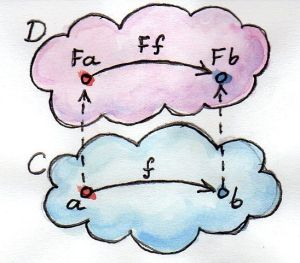
\includegraphics[scale=.5]{functor}
\end{minipage}
\begin{minipage}{.24\columnwidth}
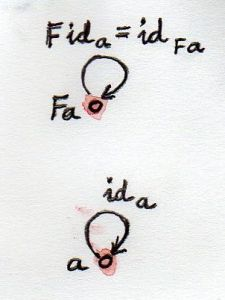
\includegraphics[scale=.5]{functorid}
\end{minipage}
\begin{minipage}{.24\columnwidth}
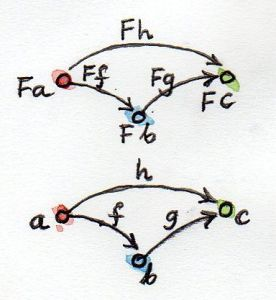
\includegraphics[scale=.5]{functorcompos}
\end{minipage}
\begin{minipage}{.24\columnwidth}
\href{https://bartoszmilewski.com/2015/01/20/functors/}{Bartosz Milewski --- Functors}
\end{minipage}


\end{frame}

\begin{frame}[fragile]{Functori în Haskell}

\structure{În general} un functor $F : \mathbb{C} \rightarrow \mathbb{D}$ este dat de
\begin{itemize}
\item O funcție $F : |\mathbb{C}| \rightarrow |\mathbb{D}|$ de la obiectele lui $\mathbb{C}$ la cele ale lui $\mathbb{D}$
\item Pentru orice $A,B \in |\mathbb{C}|$, o funcție $F : \mathbb{C}(A,B) \rightarrow \mathbb{D}(F(A),F(B))$
\item Compatibilă cu identitățile și cu compunerea
\begin{itemize}
\item $F({\it id}_A) = {\it id}_{F(A)}$ pentru orice $A$
\item $F(g\circ f) = F(g)\circ F(f)$ pentru orice $f : A \rightarrow B,g: B \rightarrow C$, $h = g\circ f$
\end{itemize}
\end{itemize}

\vfill
\structure{În Haskell}
 o instanță \lstinline$Functor f$ este dată de
\begin{itemize}
\item Un tip \lstinline$f a$ pentru orice tip \lstinline$a$ (deci \lstinline$f$ trebuie sa fie tip parametrizat)
\item Pentru orice două tipuri \lstinline$a$ și \lstinline$b$, o funcție 
\begin{asciihs}
fmap :: (a -> b) -> (f a -> f b)
\end{asciihs}
\item Compatibilă cu identitățile și cu compunerea
\begin{asciihs}
fmap id == id
fmap (g . f) == fmap g . fmap f 
\end{asciihs}
\hfill pentru orice \lstinline$f :: a -> b$ și \lstinline$g :: b -> c$
\end{itemize}
\end{frame}


\section{Functori aplicativi}

\begin{frame}{Problemă}
\begin{itemize}
\item Folosind \lstinline$fmap$ putem transforma o funcție \lstinline$h :: a -> b$ într-o funcție între cutii/computații \lstinline$fmap h :: f a -> f b$
\item Dar ce se întâmplă dacă avem o funcție cu mai multe argumente

E.g., cum trecem de la \lstinline$h :: a -> b -> c$   la \lstinline$h' :: f a -> f b -> f c$

\item putem încerca să folosim \lstinline$fmap$

\onslide<2>
\item Dar, deoarece \lstinline$h :: a -> (b -> c)$, avem că 
\lstinline$fmap h :: f a -> f (b -> c)$

\item Putem aplica \lstinline$fmap h$ la o valoare \lstinline$fa :: f a$ și obținem
\lstinline$fmap h fa :: f (b -> c)$

\item \alert{Problemă:} Cum transformăm o cutie care conține o funcție într-o funcție între cutii

\item Dacă avem asta, putem transforma funcții cu oricâte argumente.
\end{itemize}
\end{frame}

\begin{frame}[fragile]{Clasa de tipuri Applicative}
\begin{block}{Definiție}{}
\vspace{-2ex}
\begin{asciihs}
class Functor f => Applicative f where
   pure :: a -> f a
  (<*>) :: f (a -> b) -> f a -> f b
\end{asciihs}

\begin{itemize}
\item Orice instanță a lui \lstinline$Applicative$ trebuie să fie instanță a lui \lstinline$Functor$
\item \structure{\lstinline$pure$} transformă o valoare într-o computație minimală care are acea valoare ca rezultat, și nimic mai mult!
\item \structure{\lstinline$(<*>)$} ia o computație care produce funcții și o computație care produce argumente pentru funcții și obține  o computație care produce rezultatele aplicării funcțiilor asupra argumentelor
\end{itemize}
\end{block}

\begin{block}{Proprietate importantă}
\begin{itemize}
\item \lstinline$fmap f x == pure f <*> x$

\item Se definește operatorul \lstinline"(<$>)" prin  \lstinline"(<$>) = fmap"
\end{itemize}
\end{block}

\end{frame}

\begin{frame}[fragile]{Clasa de tipuri Applicative}{Instanțe}
\begin{asciihs}
class Functor f => Applicative f where
   pure :: a -> f a
  (<*>) :: f (a -> b) -> f a -> f b
\end{asciihs}

\begin{block}{Instanță pentru tipul opțiune}
\vspace{-2ex}
\onslide<2>
\begin{asciihs}
instance Applicative Maybe where
  pure = Just
  Nothing <*> _ = Nothing
  Just f  <*> x = fmap f x
\end{asciihs}
\end{block}

\onslide<1->
\begin{block}{Instanță pentru tipul eroare}
\vspace{-2ex}
\onslide<2>
\begin{asciihs}
instance Applicative (Either a) where
  pure = Right
  Left e <*> _ = Left e
  Right f  <*> x = fmap f x
\end{asciihs}
\end{block}
\end{frame}

\begin{frame}[fragile]{Clasa de tipuri Applicative}{Instanțe}
\begin{asciihs}
class Functor f => Applicative f where
   pure :: a -> f a
  (<*>) :: f (a -> b) -> f a -> f b
\end{asciihs}

\begin{block}{Instanță pentru tipul computațiilor nedeterministe (liste)}
\vspace{-2ex}
\onslide<2>
\begin{asciihs}
instance Applicative [] where
  pure x = [x]
  fs  <*> xs = [f x | f <- fs, x <- xs]
\end{asciihs}
\end{block}

\onslide<1->
\begin{block}{Instanță pentru tipul computațiilor I/O}
\vspace{-2ex}
\onslide<2>
\begin{asciihs}
instance Applicative IO where
  pure = return
  iof <*> iox = do
    f <- iof
    x <- iox
    return (f x)
\end{asciihs}
\end{block}
\end{frame}

\begin{frame}[fragile]{Clasa de tipuri Applicative}{Instanțe}
\begin{asciihs}
class Functor f => Applicative f where
   pure :: a -> f a
  (<*>) :: f (a -> b) -> f a -> f b
\end{asciihs}

\begin{block}{Instanță pentru tipul funcțiilor de sursă dată}
\vspace{-2ex}
\onslide<2>
\begin{asciihs}
instance Applicative ((->) t) where
  pure :: a -> (t -> a)
  pure x = \ _ -> x
  (<*>) :: (t -> (a -> b)) -> (t -> a) -> (t -> b)
  f  <*> g = \ x -> f x (g x)
\end{asciihs}
\end{block}

\end{frame}

\begin{frame}[fragile]{Clasa de tipuri Applicative}{Exemple}
\begin{asciihs}
Main> pure "Hey" :: [String]

Main> pure "Hey" :: Maybe String

Main> [(*0),(+100),(^2)] <*> [1,2,3]

Main> [(+),(*)] <*> [1,2] <*> [3,4]  

Main> (++) <$> ["ha","heh","hm"] <*> ["?","!","."]  

Main> filter (>50) $ (*) <$> [2,5,10] <*> [8,10,11] 

Main> (++) <$> getLine <*> getLine >>= putStrLn 
hello
 world!

\end{asciihs}
\end{frame}


\begin{frame}[fragile]{ZipList}

Idee: în loc să privim listele ca computații nedeterministe, le privim ca fluxuri de date.

\begin{asciihs}
newtype ZipList a = ZipList { getZipList :: [a]}

instance Functor ZipList where
  fmap f (ZipList xs) = ZipList (fmap f xs)
  
instance Applicative ZipList where
  pure x = repeat x
  ZipList fs <*> ZipList xs = 
    ZipList (zipWith (\ f x -> f x) fs xs)
\end{asciihs}


\end{frame}

\begin{frame}[fragile]{ZipList}{Exemple}
\begin{asciihs}
Main> getZipList $ (+) <$> ZipList [1,2,3] <*> ZipList [100,100,100]  
[101,102,103]  
Main> getZipList $ (+) <$> ZipList [1,2,3] <*> ZipList [100,100..]  
[101,102,103]  
Main> getZipList $ max <$> ZipList [1,2,3,4,5,3] <*> ZipList [5,3,1,2]  
[5,3,3,4]  
Main> getZipList $ (,,) <$> ZipList "dog" <*> ZipList "cat" <*> ZipList "rat"  
[('d','c','r'),('o','a','a'),('g','t','t')]  
\end{asciihs}
\end{frame}

\begin{frame}{Proprietăți ale functorilor aplicativi}
\begin{description}
\item[identitate] \lstinline"pure id <*> v = v"
\item[compoziție] \lstinline"pure (.) <*> u <*> v <*> w = u <*> (v <*> w)"
\item[homomorfism] \lstinline"pure f <*> pure x = pure (f x)"
\item[interschimbare] \lstinline"u <*> pure y = pure ($ y) <*> u"
\end{description}

\structure{Consecință}: \lstinline"fmap f x == f <$> x == pure f <*> x"
\end{frame}

%\begin{frame}{Categorii neasemănătoare lui $\mathrm{\mathbb{S}et}$}
%{Categoria unui graf $(V,E)$}
%\begin{itemize}
%\item Obiecte: \only<2>{varfurile grafului $V$}
%\item Săgeți: \only<2>{drumuri în grafuri}
%\item Identități:  \only<2>{drumul vid de la un vârf la el însuși}
%\item Compunere: \only<2>{alipirea drumurilor}
%\end{itemize}
%\end{frame}
%
%\begin{frame}{Categorii neasemănătoare lui $\mathrm{\mathbb{S}et}$}
%{Categoria unei relații parțiale de ordine $(S,\leq)$}
%\begin{itemize}
%\item Obiecte: \only<2>{elementele lui S}
%\item Săgeți: \only<2>{perechile $(a,b)$ din $\leq$}
%\item Identități:  \only<2>{garantate de reflexivitate}
%\item Compunere: \only<2>{garantată de tranzitivitate}
%\end{itemize}
%\end{frame}
%
%\begin{frame}{Categorii neasemănătoare lui $\mathrm{\mathbb{S}et}$}
%{Categoria asociată unui monoid $(M,\cdot, e)$}
%\begin{itemize}
%\item Obiecte: \only<2->{un singur obiect, să-l numim $m$}
%\item Săgeți: \only<2->{Elementele lui $M$}
%\item Identități:  \only<2->{$e$}
%\item Compunere: \only<2->{$\cdot$}
%\end{itemize}
%
%\onslide<3->
%\vfill 
%De fapt, merge și invers\dots
%
%\begin{block}{Monoidul asociat unei categorii cu un singur obiect $|\mathbb{C}|=\{m\}$}
%\begin{itemize}
%\item $M = \mathbb{C} = \mathbb{C}(m,m)$
%\item $\cdot = \circ$
%\item $e = \mathit{id}_m$
%\end{itemize}
%\end{block}
%\end{frame}
%

\section{Monoizi}

\begin{frame}[fragile]{Monoizi}{Data.Monoid.Monoid}
\begin{asciihs}
class Monoid m where
    mempty  :: m
    mappend :: m -> m -> m
\end{asciihs}

\begin{block}{Monoidul listelor}
\vspace{-2ex}
\begin{asciihs}
instance Monoid [a] where
    mempty  = []
    mappend = (++)
\end{asciihs}
\end{block}
\end{frame}


\begin{frame}[fragile]{Monoide booleene}
\begin{block}{Monoidul conjunctiv\hfill Data.Monoid.All}
\vspace{-2ex}
\begin{asciihs}
newtype All = All { getAll :: Bool }

instance Monoid All where
        mempty = All True
        All x `mappend` All y = All (x && y)
\end{asciihs}
\end{block}
\begin{block}{Monoidul disjunctiv\hfill Data.Monoid.Any}
\vspace{-2ex}
\begin{asciihs}
newtype Any = Any { getAny :: Bool }

instance Monoid Any where
        mempty = Any False
        Any x `mappend` Any y = Any (x || y)
\end{asciihs}
\end{block}
\end{frame}


\begin{frame}[fragile]{Monoide numerice}
\begin{block}{Monoidul aditiv\hfill Data.Monoid.Sum}
\vspace{-2ex}
\begin{asciihs}
newtype Sum a = Sum { getSum :: a }

instance Num a => Monoid (Sum a) where
        mempty = Sum 0
        Sum x `mappend` Sum y = Sum (x + y)
\end{asciihs}
\end{block}
\begin{block}{Monoidul multiplicativ\hfill Data.Monoid.Product}
\vspace{-2ex}
\begin{asciihs}
newtype Product a = Product { getProduct :: a }

instance Num a => Monoid (Product a) where
        mempty = Product 1
        Product x `mappend` Product y = Product (x * y)
\end{asciihs}
\end{block}
\end{frame}


\begin{frame}[fragile]{La ce sunt buni Monoizii?}
{Data.Foldable.foldMap}
\begin{itemize}
\item Agregare într-un monoid:
\begin{asciihs}
    foldMap :: Monoid m => (a -> m) -> [a] -> m
    foldMap f = foldr (mappend . f) mempty
\end{asciihs}  
\end{itemize}
\begin{block}{Exemple}
\vspace{-2ex}
\begin{asciihs}
concat :: [[a]] -> [a]
concat = foldMap id
    
all :: [Bool] -> Bool         any :: [Bool] -> Bool
all = getAll . foldMap All    any = getAny . foldMap Any
    
sum :: Num a => [a] -> a      product :: Num a => [a] -> a
sum = getSum . foldMap Sum    product =
                                getProduct . foldMap Product
\end{asciihs}      
\end{block}
\end{frame}


\begin{frame}[fragile]{Monoidul endomorfismelor}
\begin{asciihs}
newtype Endo a = Endo { appEndo :: a -> a }

instance Monoid (Endo a) where
        mempty = Endo id
        Endo f `mappend` Endo g = Endo (f . g)
\end{asciihs}
\begin{itemize}
\item Mulțimea funcțiilor din $A$ în $A$ are structură de monoid
\end{itemize}
\end{frame}

\begin{frame}[fragile]{Relația între foldr și foldMap}
\begin{block}{foldMap în funcție de foldr}
\begin{asciihs}
    foldMap :: Monoid m => (a -> m) -> [a] -> m
    foldMap f = foldr (mappend . f) mempty
\end{asciihs}  
\end{block}

\begin{block}{foldr în funcție de foldMap}
\begin{asciihs}
    foldr :: (a -> b -> b) -> b -> [a] -> b
    foldr f z t = appEndo (foldMap (Endo . f) t) z
\end{asciihs}  

\structure{Observație:} \lstinline$f :: a -> (b -> b)$ translatează un element din a într-un endomorfism peste b
\end{block}
\end{frame}

%\section{Obiecte speciale într-o categorie}
%
%\begin{frame}[fragile]{Obiecte inițiale și finale}
%\begin{block}{Obiect inițial}
%Un obiect din care \structure{există} un \structure{singur} morfism către orice alt obiect
%\begin{itemize}
%\item mulțimea vidă în categoria Set
%\item Algebra de termeni peste o signatură
%\end{itemize}
%\end{block}
%\begin{block}{Obiect final}
%Un obiect către care \structure{există} un \structure{singur} morfism din orice alt obiect
%\begin{itemize}
%\item O mulțime singleton în categoria Set
%\item Algebra în care suportul fiecărui sort e singleton
%\item Tipul \structure{()} în Hask
%
%Pentru orice tip a, există o singură funcție de la a în ()
%\begin{asciihs}
%    unit :: a -> ()
%    unit _ = ()
%\end{asciihs}
%\end{itemize}
%\end{block}
%\end{frame}
%
%\section{Dualitate}
%
%\begin{frame}{Duala unei categorii}
%Dată fiind categoria $\mathbb{C}$, putem defini duala ei $\mathbb{C}^{op}$, prin simpla inversare a direcțiiei săgeților, astfel:
%\begin{itemize}
%\item $|\mathbb{C}^{op}|$ = $|\mathbb{C}|$
%\hfill $\mathbb{C}^{op}$ = $\mathbb{C}$
%\hfill $\mathit{dom}_{\mathbb{C}^{op}} = \mathit{codom}_{\mathbb{C}}$
%\hfill $\mathit{codom}_{\mathbb{C}^{op}} = \mathit{dom}_{\mathbb{C}}$
%\item $\circ_{\mathbb{C}^{op}} : \mathbb{C}^{op}(B,C) \times \mathbb{C}^{op}(A,B) \rightarrow \mathbb{C}^{op}(A,C)$ dată de:
%
%pentru $f\in \mathbb{C}^{op}(B,C) = \mathbb{C}(C,B)$ și  $g\in \mathbb{C}^{op}(A,B) = \mathbb{C}(B,A)$, definim 
%$$f \circ_{\mathbb{C}^{op}} g = g \circ_{\mathbb{C}} f \in  \mathbb{C}(C,A) = \mathbb{C}^{op}(A,C)$$
%\item Identitățile rămân aceleași
%\item Se verifică proprietățile de asociativitate
%\end{itemize}
%
%\begin{block}{Orice proprietate poate fi dualizată}
%\begin{itemize}
%\item Obiect final este obiect inițial în categoria duală
%\item Obiect inițial este obiect final în categoria duală
%\end{itemize}
%\end{block}
%\end{frame}
%
%\section{Izomorfism}
%
%\begin{frame}[fragile]{Izomorfism. Obiecte izomorfe}
%Un morfism \lstinline$f :: A -> B$ se numește \structure{izomorfism}
%dacă există un morfism \lstinline$g :: B -> A$ astfel încât
%\vspace{-1ex}
%\begin{asciihs}
%f . g = id :: B -> B
%g . f = id :: A -> A
%\end{asciihs}
%În acest caz, și g este izomorfism, iare obiectele A și B se numesc izomorfe
%
%
%\begin{block}{Teoremă: Obiectul inițial e unic (modulo izomorfisme)}
%\onslide<2>
%Adică, oricare două obiecte inițiale într-o categorie sunt izomorfe
%
%Fie A și B inițiale.  Atunci există (unice) \lstinline$f :: A -> B$ și \lstinline$g :: B -> A$. Avem:
%\vspace{-1ex}
%\begin{asciihs}
%f . g :: B -> B                             id :: B -> B
%g . f :: A -> A                             id :: A -> A
%\end{asciihs}
%Din unicitatea morfismelor de la A în A și B în B, rezultă
%\vspace{-1ex}
%\begin{asciihs}
%f . g = id :: B -> B
%g . f = id :: A -> A
%\end{asciihs}
%\end{block}
%\structure{Din dualitate și obiectul final e unic (modulo izomorfime)}
%
%\end{frame}
%
%\section{Produse și coproduse}
%
%
%\begin{frame}[fragile]{Produs}
%Produsul a două obiecte a și b este obiectul c înzestrat cu două proiecții 
%\lstinline$pa :: c -> a$ și \lstinline$pb :: c -> b$ astfel încât pentru orice alt obiect c' înzestrat cu două proiecții \lstinline$pa' :: c' -> a$ și \lstinline$pb' :: c' -> b$, există un unic morfism \lstinline$m :: c' -> c$ care factorizează aceste proiecții, adică:
%\vspace{-1ex}
%\onslide<2>
%\begin{asciihs}
%m . pa = pa'                                   m . pb = pb'
%
%type Product a b = (a,b)
%pa :: Product a b -> a
%pa = fst
%pb :: Product a b -> b
%pb = snd
%
%-- Factorizarea
%factor  :: (c -> a) -> (c -> b) -> (c -> Product a b)
%factor pa' pb' x = (pa' x, pb' x)
%
%-- Avem
%fst . factor pa' pb' = pa'        snd . factor pa' pb' = pb'
%\end{asciihs}
%\end{frame}
%
%
%\begin{frame}[fragile]{Coproduse}
%Coprodusul a două obiecte a și b este produsul lor în categoria duală, adică obiectul c înzestrat cu două injecții 
%\lstinline$ia :: a -> ca$ și \lstinline$ib :: b -> c$ astfel încât pentru orice alt obiect c' înzestrat cu două injecții \lstinline$ia' :: a -> c'$ și \lstinline$ib' :: b -> c'$, există un unic morfism \lstinline$m :: c' -> c$ care factorizează aceste injecții, adică \lstinline$ia . m = ia'$ și \lstinline$ib . m = ib'$
%\vspace{-1ex}
%\onslide<2>
%\begin{asciihs}
%type Sum a b = Left a | Right b
%ia :: a -> Sum a b
%ia = Left
%ib :: b -> Sum a b
%ib = Right
%
%-- Factorizarea
%factor  :: (a -> c) -> (b -> c) -> (Sum a b -> c)
%factor ia' ib' (Left x) = ia' x
%factor ia' ib' (Right x) = ib' x
%-- Avem
%factor ia' ib' . ia = ia'        factor ia' ib' . ib = ib'
%\end{asciihs}
%\end{frame}

\end{document}



